%%%%%%%%%%%%%%%%%%%%%%%%%%%%%%%%%%%%%%%%%%%%%%%%%%%%%%%%%%%%%%%%%%%%%%%%%%%%%%%%%%%%%%%%%%%%%%%%%%%%%%%%%%%%%%%%%%%%%%%%%%%%%%%%%%%%%%%%%%%%%%%%%%%%%%%%%%%
% This is just an example/guide for you to refer to when submitting manuscripts to Frontiers, it is not mandatory to use Frontiers .cls files nor frontiers.tex  %
% This will only generate the Manuscript, the final article will be typeset by Frontiers after acceptance.   
%                                              %
%                                                                                                                                                         %
% When submitting your files, remember to upload this *tex file, the pdf generated with it, the *bib file (if bibliography is not within the *tex) and all the figures.
%%%%%%%%%%%%%%%%%%%%%%%%%%%%%%%%%%%%%%%%%%%%%%%%%%%%%%%%%%%%%%%%%%%%%%%%%%%%%%%%%%%%%%%%%%%%%%%%%%%%%%%%%%%%%%%%%%%%%%%%%%%%%%%%%%%%%%%%%%%%%%%%%%%%%%%%%%%

%%% Version 3.4 Generated 2022/06/14 %%%
%%% You will need to have the following packages installed: datetime, fmtcount, etoolbox, fcprefix, which are normally inlcuded in WinEdt. %%%
%%% In http://www.ctan.org/ you can find the packages and how to install them, if necessary. %%%
%%%  NB logo1.jpg is required in the path in order to correctly compile front page header %%%

\documentclass[utf8]{FrontiersinHarvard} % for articles in journals using the Harvard Referencing Style (Author-Date), for Frontiers Reference Styles by Journal: https://zendesk.frontiersin.org/hc/en-us/articles/360017860337-Frontiers-Reference-Styles-by-Journal
%\documentclass[utf8]{FrontiersinVancouver} % for articles in journals using the Vancouver Reference Style (Numbered), for Frontiers Reference Styles by Journal: https://zendesk.frontiersin.org/hc/en-us/articles/360017860337-Frontiers-Reference-Styles-by-Journal
%\documentclass[utf8]{frontiersinFPHY_FAMS} % Vancouver Reference Style (Numbered) for articles in the journals "Frontiers in Physics" and "Frontiers in Applied Mathematics and Statistics" 

%\setcitestyle{square} % for articles in the journals "Frontiers in Physics" and "Frontiers in Applied Mathematics and Statistics" 
\usepackage{url,hyperref,lineno,microtype,subcaption}
\usepackage[onehalfspacing]{setspace}

\newcommand{\appname}{\emph{Discourse2Draft}}
\newcommand{\maxTokensSummarization}{500}
\newcommand{\chunkWindowSize}{1,000}
\newcommand{\chunkWindowOverlap}{200}
\newcommand{\numKeyPhrases}{10}
\newcommand{\numDocsRAG}{5}
\newcommand{\numKeyPhrasesLitSearch}{5}
\newcommand{\maxContentSizePerLiterature}{20000}
\newcommand{\maxNumLiterature}{2}

\linenumbers


% Leave a blank line between paragraphs instead of using \\


\def\keyFont{\fontsize{8}{11}\helveticabold }
\def\firstAuthorLast{Talukder {et~al.}} %use et al only if is more than 1 author
\def\Authors{Amlan Talukder\,$^{1,3*}$, Parker K. Combs\,$^{2,4}$, Charles P. Schmitt\,$^{3}$, David M. Reif\,$^{2}$ and Scott S. Auerbach\,$^{2}$}
% Affiliations should be keyed to the author's name with superscript numbers and be listed as follows: Laboratory, Institute, Department, Organization, City, State abbreviation (USA, Canada, Australia), and Country (without detailed address information such as city zip codes or street names).
% If one of the authors has a change of address, list the new address below the correspondence details using a superscript symbol and use the same symbol to indicate the author in the author list.
\def\Address{$^{1}$ Office of Data Science (ODS), NIH/NIEHS, Durham, NC, United States \\
$^{2}$ Predictive Toxicology Branch (PTB), Department of Translational Toxicology (DTT), NIH/NIEHS, Durham, NC, United States \\
$^{3}$ 22nd Century Technologies, McLean, VA, United States \\
$^{4}$ Axle Informatics, Rockville, MD, United States}
% The Corresponding Author should be marked with an asterisk
% Provide the exact contact address (this time including street name and city zip code) and email of the corresponding author
\def\corrAuthor{Amlan Talukder}

\def\corrEmail{amlan.talukder@nih.gov}


\begin{document}
\onecolumn
\firstpage{1}

\title[Discourse2Draft]{Discourse2Draft: An AI powered structured document writing tool} 

\author[\firstAuthorLast ]{\Authors} %This field will be automatically populated
\address{} %This field will be automatically populated
\correspondance{} %This field will be automatically populated

\extraAuth{}% If there are more than 1 corresponding author, comment this line and uncomment the next one.
%\extraAuth{corresponding Author2 \\ Laboratory X2, Institute X2, Department X2, Organization X2, Street X2, City X2 , State XX2 (only USA, Canada and Australia), Zip Code2, X2 Country X2, email2@uni2.edu}


\maketitle

\begin{abstract}

%%% Leave the Abstract empty if your article does not require one, please see the Summary Table for full details.
We introduce \appname{}, a model-agnostic, retrieval-augmented generation (RAG) based application that converts a user-provided query into an exhaustive structured outline and, from that outline, into a polished long-form draft, using context from either user provided documents or literature downloaded from \emph{PubMed} or both. The system can also take the structured outline directly from the user. The system extracts the hierarchical structure from the outline (either AI-generated or user provided) and detects positions to write contents. It then orchestrates prompts to large-language models (LLMs) to extract core ideas from the corresponding section headers and previously written text for every writable position, fill that position with cohesive prose with context taken from user provided documents or online literature, and automatically weave source-anchored citations throughout the text. The draft with associated references and the bibliography can be exported in docx, LaTex and Markdown formats, ensuring full transparency and downstream editability. By coupling multi-vendor LLM flexibility with traceable knowledge retrieval and granular certainty metrics, \appname{} streamlines the journey from informal textual query to publication-quality writing while keeping scientific rigor and author oversight at the forefront. 


\tiny
 \keyFont{ \section{Keywords:} Document Writing, Deep Research, RAG, LLM, AI, AI Workflow} %All article types: you may provide up to 8 keywords; at least 5 are mandatory.
\end{abstract}

\section{Introduction}

The rapid proliferation of large-language models (LLMs) has catalyzed a new generation of “deep research” platforms that promise to accelerate literature discovery, hypothesis generation, and scientific writing. Tools such as Semantic Scholar’s TLDR feature (\citep{Cachola2020TLDRES}), Elicit’s question-answering workflow (\citep{elicit2023}), Research Rabbit’s citation-network visualizations (\citep{researchrabbit2025}), and Scholarcy’s automated paper digests (\citep{scholarcy2026}) exemplify the growing ecosystem of systems that summarize findings, surface related work, or extract structured information from vast corpora. More recently, retrieval-augmented generation (RAG) frameworks—including GitHub Copilot for code and Scite’s Smart Citation Generator (\citep{nicholson2021scite})—have blended local knowledge bases with generative text to create context-aware outputs that more closely mimic domain expertise. Despite these advances, most existing solutions fail to provide a structured outline as per user intention and authentic references to the content. Many of these tools focus on gathering basic literature information (title and abstract) on a topic, often powered by a simple internet search and/or limited number of document summarization or narrow task support; few enable researchers to generate full, publication-grade manuscripts with structured user provided outline while preserving traceability to source material and providing explicit measures of factual certainty.

\appname{} addresses this gap by offering an open-source, end-to-end, query-to-manuscript pipeline that is simultaneously transparent, customizable, and model-agnostic. It provides full control on the outline of a manuscript (or any structured document) and proper content citations of authentic publications downloaded from a rich and trusted literature database, \emph{PubMed}. After ingesting a user-supplied query, the application uses LLM to shape an outline for the manuscript. It then writes each section of the outline using relevant information from user-provided documents or literature from \emph{PubMed} or both as LLM context using RAG approach. \appname{} also exposes granular controls like domain, writing style, size of the written document which should allow authors to modulate both the breadth and depth of the output. By coupling controls on both structure and content of a document with authentic references, \appname{} empowers scientists to tailor AI-generated manuscripts to diverse journal formats, grant applications, or internal reports without sacrificing rigor or authorial oversight. \appname{} also provides manageability by allowing users to regenerate sections as needed and download the output and references in the popular varieties of editable document formats.

\section{Methods}

\subsection{User account and settings}
\appname{} can be accessed without creating an account. But a user account is helpful to store the generated and uploaded documents and associated settings. The settings include API key and URL of the LLM provider, temperature of the LLM and generic instructions for the content generation.

\subsection{User inputs}

\subsubsection{Query and outline}
\appname{} offers flexibility in terms of user interactions. As an input, it takes either a user query (e.g. Write a review article on Quantum Computing.) or a structured outline of the draft following a set of rules mentioned in the next paragraph. With structured outline, user has more control on the generated content as it strictly follows the user provided outline. If a user query is provided as input, it first creates a structured outline and then starts writing the content. So, creating a structured outline is the first essential step in \appname{}. The user can make changes to the generated outline with an interactive user interface (UI). 

\textbf{Query tab:} User can provide a query and upload with an reference file (if necessary). Next step is to click the ``Create outline" button, which will generate a structured outline on the query considering the reference file (if provided). 

\textbf{Structured Outline tab:} User can directly provide a structured outline following \appname{} provided guidelines. This helps the AI model to parse the structured outline and identify places where it needs to generate contents. It also helps the AI model to extract the pre-written summary of the content which will be useful to maintain the continuity in generating the new content. 

\textbf{Structured Outline Guidelines:} The structured outline must maintain the standard Markdown section hierarchy with the number of ``\#"s, where the each hierarchy level header is preceded by ``\#"s. One ``\#" means the topmost level (which typically is the title of the outline) and consistent increment in the number of ``\#"s would ensure the sub-levels, e.g. two ``\#"s mean the second level hierarchy (e.g. Abstract, Introduction etc.) and so on. An outline must begin with one ``\#" (top-level hierarchy). The position where the AI needs to write the content has to be specified with a ``$<$content$>$" tag. User can add additional instructions for content generation under each section (or sub-section etc.) enclosing the instructions within ``$<$Instructions$>$" and ``$<$/Instructions$>$" tags (Fig. \ref{fig:outline_format}).



\subsubsection{Document upload}
\appname{} has the facility to use user-uploaded documents during content generation. The documents can be uploaded as ``text (TXT)", ``Microsoft Word (DOCX)" or ``PDF" formats from the user machine on the ``Upload documents" panel in the bottom left corner of the UI. The uploaded documents can later be attached to a new file for content generation. The uploaded documents ids are stored in a relational database associated with the user account (if the user signed in) or the active session (if the user did not sign in).

\subsection{Content generation}

\subsubsection{Outline processing}
To write a document, \appname{} either takes a structured outline from the user or creates one based on the user provided query. It then breaks the outline into a hierarchical structure (Fig. \ref{fig:outline_format}), validates it and detects the first position in the outline where it needs to write (denoted by the ``$<$content$>$" tag). It then gathers the header chain specified by ``\#"s of that position from the topmost level (title $\rightarrow$ section $\rightarrow$ subsection $\rightarrow$ sub-subsection etc.) and the generated contents so far to ensure the relevance and consistency in content generation. It also gathers the instructions for the corresponding section, if it is provided within ``$<$Instructions$>$" and ``$<$/Instructions$>$" tags. It then detects if the outline has an ``Abstract" section or a section with a similar header e.g. ``Summary", ``Synopsis", ``Outline" etc. \appname{} does this detection with an AI call. If the writable position is part of an ``Abstract" section, it saves it to write at the end and move on to the next section. To write in a position, \appname{} passes the corresponding section header chain and the summary of the previous contents to a suitable AI workflow (described later in this section). AI model generates the content and a document content summary up to the current position, which can be used to generate the next content (Fig. \ref{fig:ai_workflow}).

\subsubsection{AI workflows for content generation}

\appname{} follows different AI workflow based on user needs (Fig. \ref{fig:ai_workflow}). Each workflow uses three inputs; the section header chain of the current position, the summary of the previously written contents and user-provided instructions for this section extracted from the ``$<$Instructions$>$" and ``$<$/Instructions$>$" tags. Each workflow generates two outputs; the AI-generated content and the summary of the overall content (joins the generated content with the previous content summary). In the beginning of an AI workflow, it summarizes the previously written contents, if it contains over \maxTokensSummarization{} tokens to ensure that the number of context-tokens does not exceed the limit of underlying LLM. This step is usually redundant as the input already considers the summarized version of the previously written content. But if the AI fails to summarize the content in the last step, this step helps to double check and keep the number of tokens within the threshold.

\textbf{Basic:} This workflow generates content from the training data of associated LLM, based on the headers and previously written content summary. This workflow is used as default.

\textbf{RAG:} This workflow considers context from user provided documents. When a user provided document is attached to this workflow, the document is first divided into chunks of \chunkWindowSize{} characters of text with an overlap of \chunkWindowOverlap{} characters and then each chunk of text is converted into an embedding vector (called ``vector document") and saved into a vector database table (called ``collection"), here we refer it as \emph{document collection}. To generate content for a file with attached user documents, \appname{} follows the ``RAG" workflow, where the underlying LLM analyzes the previous content summary and current section headers to generate \numKeyPhrases{} semantically independent key-phrases relevant to the topic. Then each key-phrase is searched in the vector database collection to find \numDocsRAG{} semantically similar ``vector documents". The key-phrases and the retrieved texts from the ``vector documents" are combined and passed to the LLM as context. Finally, LLM considers the provided context along with its training data to generate the final content.

\textbf{Literature:} Apart from the user uploaded documents, \appname{} also has the ability to gather content from online literature database. This ability is turned on by setting ``Literature Search" on at the top of the content panel (Fig. \ref{fig:app_screenshot}). After that, \appname{} continues the similar steps in the ``RAG" workflow, but replaces the vector database search with literature search. Similar to ``RAG" workflow, it starts with analyzing the previous content summary and the current section header to generate \numKeyPhrasesLitSearch{} key-phrases, uses each key-phrase to query against the online literature database, picks \maxNumLiterature{} best match articles and extracts the first \maxContentSizePerLiterature{} number of letters from each article. In this version of \appname{}, we only use the open access \emph{PubMed Central} database as the literature database (\citep{roberts2001pubmed}). The extracted contents of the literature is then processed in the same way as the ``RAG" workflow and saved in the vector database collection, which we refer here as (\emph{literature collection}). The rest of the steps are the same as the ``RAG" workflow.

\textbf{RAG + Literature:} This workflow, as the name suggests, merges both ``RAG" and ``Literature" workflows. Here each key-phrase, generated after analyzing the previous contents and the current section headers, will be used for both searching the \emph{document collection} and the \emph{literature collection} of the vector database to retrieve semantically similar text chunks from both sources. The text chunks are then passed to the LLM as context. In this way, the LLM considers the provided context from both uploaded documents and relevant literature search along with its training data to generate the final content.

\subsubsection{Other AI workflows}

Other than content generation, \appname{} uses AI workflows in outline generation and formatting and abstract detection and writing. These workflows are relatively simpler than the content generation workflows and are driven mainly with prompt engineering. The outline generation workflow works when the user provides a text based query, as input, with or without the reference file. If a reference file is provided with the query, the outline generation workflow iteratively summarizes the content from the reference file and extracts the gist that fits within LLM context token limit. When the user provides the structured outline directly as input, the outline formatter workflow is used to fix the outline, if needed. The abstract detection workflow is applied to find if the outline has an ``Abstract" or a section with similar header e.g. ``Summary", ``Synopsis", ``Outline" etc. If there is an abstract, \appname{} writes it using the abstract writer workflow after the entire document is written.

\subsubsection{Referencing}
When either of ``RAG", ``Literature" and ``RAG + Literature" workflows is used, \appname{} cites the generated text with references from the user provided documents or online literature. It maintains correctness and order of every reference that is cited in the generated document. When an uploaded document is attached or a literature is searched, a record with the metadata on the document or literature is created in a relational database. In the above three workflows, LLMs use text chunks retrieved from the vector database as context to generate the final content. Each text chunk is tagged with the corresponding record identifier (id) from the relational database. Each text chunk associated with the id is provided to the LLM as context. The LLM is instructed to cite the id of a text chunk at the end of every group of sentences it generates using that text chunk. The cited id is then programmatically processed to create citation at the specified position of the content. A list of references of the cited documents and literature is shown in American Psychological Association format (APA) format at the end of the document under the ``References" section (Fig. \ref{fig:app_screenshot}). 

\subsection{Modification of content}

\appname{} provides features that allow user to modify each paragraph of the content after content generation. User can either expand or rephrase a paragraph with specific instructions or completely remove it from the content. The controls for regeneration are shown on the content bar when a paragraph is selected for modification (Fig. \ref{fig:app_screenshot}).

\subsection{Concept Map}

Each document is associated with a concept map which is a tree of key-phrases explored by AI to generate content under a section. This map should help user get an overview of the document without reading it. It should also help user validate the thoughts of the AI model during content generation (Fig. \ref{fig:concept_map}). The concept map can be accessed via the ``Concept Map" button at the top of the content panel.

\subsection{Custom instructions for AI}

\appname{} follows a set of regulation with the highest priority that are built-in as system prompt. User can add instructions on top of that in the settings menu that apply on the files generated under the user profile. As mentioned earlier, user can also add instructions inside the structured outline within ``$<$Instructions$>$" and ``$<$/Instructions$>$" tags. These instructions are section specific and are appended with the instructions provided in the user profile settings. Other than these instructions, user can also add instructions to regenerate a paragraph of a file content. These instructions are appended at the end of the other user instructions.  

\subsection{Outputs}
\appname{} provides the facility to download the generated document in Markdown (.md), Microsoft Word (.docx) and LaTex (.tex) formats. Markdown, Microsoft Word formatted files contain the references inside the file. For the LaTex formatted file, the bibliography of the associated references can be downloaded separately as ``bibtex" format. The download options are shown on the right side of the outline panel, in the generated documents panel and the expanded view of generated documents panel, which can be opened by clicking the expand button on the top right corner of the panel. The concept map of a document can be downloaded in JSON format.

\subsection{Technology Stack}
\appname{} was built using python programming language. The front-end of \appname{} was developed using python-shiny package and JavaScript. For the relational database in the back-end PostgreSQL was used. LangChain and LangGraph packages were used to create and manage the AI workflows. Chroma was used as the vector database (Fig. \ref{fig:tech_stack}).

\subsection{Installation}

\appname{} code can be downloaded from GitHub (\url{https://github.com/amlantalukder/Discourse2Draft}). The repository contains step by step instructions to install it.

\section{Evaluation}

We evaluated \appname{} by comparing it with two state-of-the-art deepresearch AI tools: \emph{OpenAI deep research} (\citep{deepresearch2025openai}) and \emph{Manus AI} (\citep{shen2025mind}) (Lite version) adopting LLM-as-a-judge approach. As documents to generate, we picked three topics from biomedical domain space; ``CRISPR-based therapeutic genome editing for inherited blood disorders", ``Phthalates Toxicity" and ``Health Impacts of Per- and Polyfluoroalkyl Substances (PFASs): A Comprehensive Review". Each of these topics are well researched in the respective domain, thus has many peer-reviewed articles in \emph{PubMed Central}. We generated contents on the three topics with the same queries for the three tools. Each query contains an outline which section hierarchy so that the tools can maintain the structure and hence can be compared with \appname{}. For \appname{}, we used the ``literature search" workflow with GPT-5, o1 and o1-mini from OpenAI as the underlying LLMs to generate the contents on the three topics in the respective order. As evaluator, we used two AI agents using o3 from OpenAI and Gemini 3.1 Pro from Google to score the contents of each section of the three documents within 0 to 100 based on the following criteria: 

\textit{Relevance:} Is the content relevant to the provided section header and the previously written content summary (if provided)?

\textit{Continuity:} Is the content writing style continuous with the previously written content summary? The highest score (100) is given if previously written content summary is not provided. This criterion is not used to score ``References".

\textit{Non-repetitiveness:} Is the content devoid of repetitiveness compared with the previously written content summary? The highest score (100) if previously written content summary is not provided.

\textit{Specificity:} Is the content devoid of hallucination? 

Across the evaluated documents, \appname{} generally maintained close alignment with section headers and thematic expectations highlighted by the \textit{relevance} scores. This indicates that \appname{} effectively interpreted the preset instructions and produced content that adheres to the intended topical scope, a critical requirement for scientific and review-style writing. \appname{} also demonstrated solid performance in maintaining \textit{continuity}, despite using a short summary on the previous content controlled with maximum tokens threshold (\maxTokensSummarization). Its outputs tended to preserve a coherent narrative flow and stylistic consistency across sections, suggesting that it effectively leverages contextual inputs. This is especially important in multi-section biomedical documents, where logical progression and conceptual linkage between sections enhance readability and scholarly quality. Although not as strong as the previous two criteria, in terms of \textit{non-repetitiveness} \appname{} appeared capable of avoiding redundant phrasing and content overlap with previously generated sections. This contributes to more concise and information-dense writing, which is desirable in technical domains where redundancy can obscure key insights.

To highlight some of the weaknesses, \appname{} exhibited limitations in specificity, particularly in complex biomedical contexts. Instances of overgeneralization and occasional hallucination-like behavior suggest that the model may struggle with grounding its outputs in precise, verifiable scientific detail. This is a critical shortcoming, as specificity and factual accuracy are paramount in biomedical writing. Another observed weakness is inconsistent performance across document sections and topics. While \appname{} performs well in structurally straightforward sections (e.g., introductions or summaries), its performance may degrade in more technically demanding sections such as mechanistic explanations or regulatory analyses. This variability suggests that the model's internal knowledge integration and reasoning depth may not be uniformly robust across domains. Although these shortcomings can be overcome by providing more information to the AI workflow. This can be done by revising the user provided instructions and/or increasing the number of tokens in the previous content summary, the number of manuscripts and the content size of each manuscript, which are \maxTokensSummarization{}, \maxNumLiterature{} and \maxContentSizePerLiterature{} respectively in the default settings. Also, \appname{} used a simplistic workflow to download literature documents from only one source (\emph{Pubmed Central}), while the other two proprietary tools use networks of agents (\citep{deepresearch2025openai, shen2025mind}) to do the deep research from a wide variety of sources from internet. Despite these limitations, \appname{} was able to maintain a competitive score on all the above-mentioned criteria, and consistently higher scores on the ``References".

\section{Discussion}

We aimed to develop an open-source, AI-powered document generation tool that can efficiently and reliably help researcher generating drafts balancing flexibility with complete content control. \appname{} can generate structured contents like other numerous tools available now or appearing everyday. But unlike most of the AI tools, it allows user to maintain control on the structure of the content. The references inserted in the content are devoid of hallucinations as they are cross-referenced and validated during content generation. \appname{} also demonstrates a balanced profile in structural alignment, coherence, and non-redundancy, making it well-suited for generating organized draft documents. However, its limitations in specificity and depth of scientific reasoning constrain its effectiveness for high-stakes biomedical writing tasks. As a future improvement, we will focus on enhancing factual grounding, reducing hallucinations, and strengthening domain-specific reasoning capabilities to better compete with leading deep research AI systems. In the current settings, the underlying workflows of \appname{} were kept simple to maintain a balance between speed and accuracy. We used \emph{PubMed Central} free full text literature database which primarily focuses on the articles published in biomedical domain. For other domains, we plan to add more online databases that provide open access to the full text of an article (e.g. Web of Science, Scopus etc.). \appname{} can serve the purpose of generating a variety of structured documents in academia e.g. manuscripts for research article, literature review, research proposals, thesis dissertation, case study, systematic review etc. The code-base is provided as open source to the community to be extended and perfected as needed.

\section*{Conflict of Interest Statement}
%All financial, commercial or other relationships that might be perceived by the academic community as representing a potential conflict of interest must be disclosed. If no such relationship exists, authors will be asked to confirm the following statement: 

The authors declare that this work was done in the absence of any commercial or financial relationships that could be construed as a potential conflict of interest.

\section*{Author Contributions}

SA and CS conceptualized the idea. PC designed and managed the AI infrastructure and database support. AT designed and implemented the tool. AT and SA contributed in manuscript writing. PC, CS and DR contributed with feedbacks and revisions.

\section*{Funding}
This research was supported by the NIH, National Institute of Environmental Health Sciences, through Intramural Research Project ZIAES103385.

\section*{Supplemental Data}
The documents generated by \emph{OpenAI deep research}, \emph{Manus AI} and \appname{} are provided as supplementary data.

 \bibliographystyle{Frontiers-Harvard} %  Many Frontiers journals use the Harvard referencing system (Author-date), to find the style and resources for the journal you are submitting to: https://zendesk.frontiersin.org/hc/en-us/articles/360017860337-Frontiers-Reference-Styles-by-Journal. For Humanities and Social Sciences articles please include page numbers in the in-text citations 
%\bibliographystyle{Frontiers-Vancouver} % Many Frontiers journals use the numbered referencing system, to find the style and resources for the journal you are submitting to: https://zendesk.frontiersin.org/hc/en-us/articles/360017860337-Frontiers-Reference-Styles-by-Journal
\bibliography{main}

\section*{Figure captions}

\begin{figure}
\centering
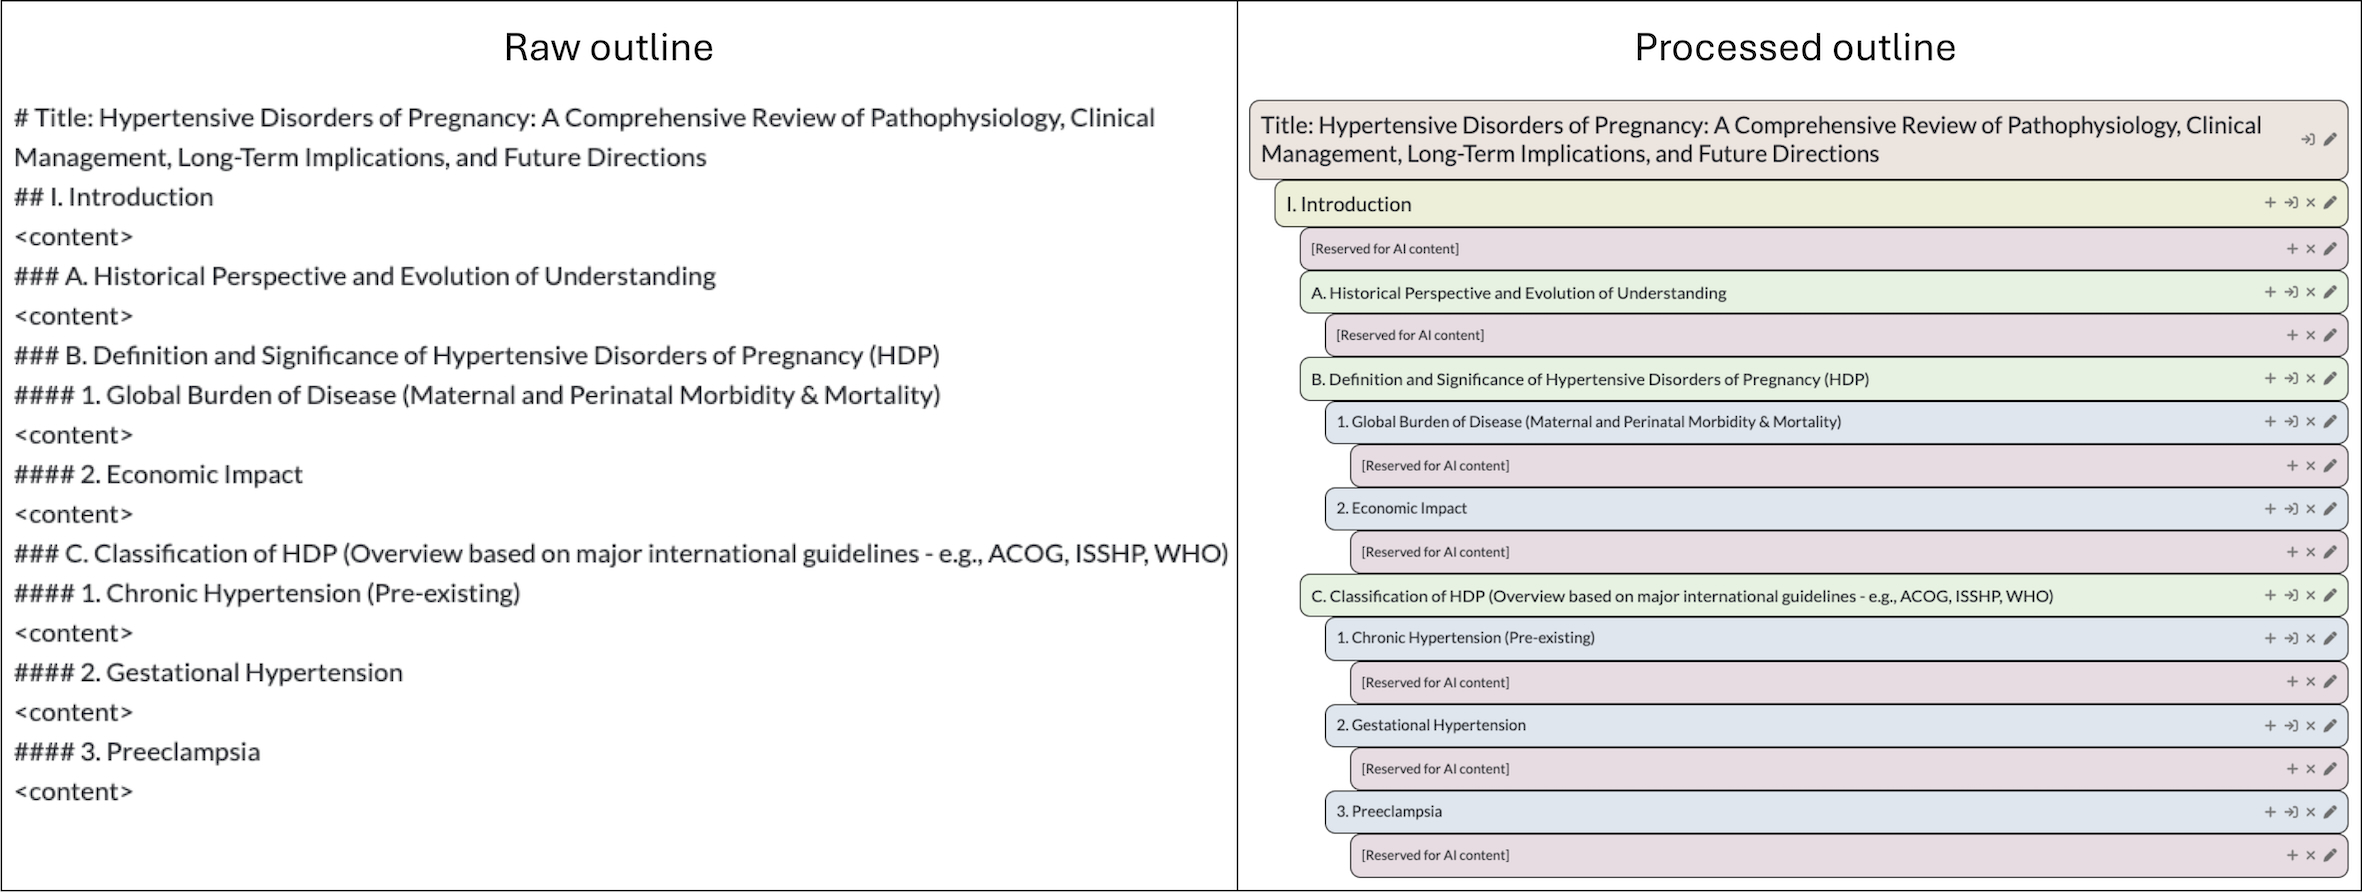
\includegraphics[width=1\linewidth]{outline_example.jpg}
\caption{\label{fig:outline_format} Raw outline input format of content creation. The left panel shows an example of the structured outline with the necessary syntax. The right panel shows the hierarchy of how the outline is processed from the raw text shown in the left panel.}
\end{figure}

\begin{figure}
\centering
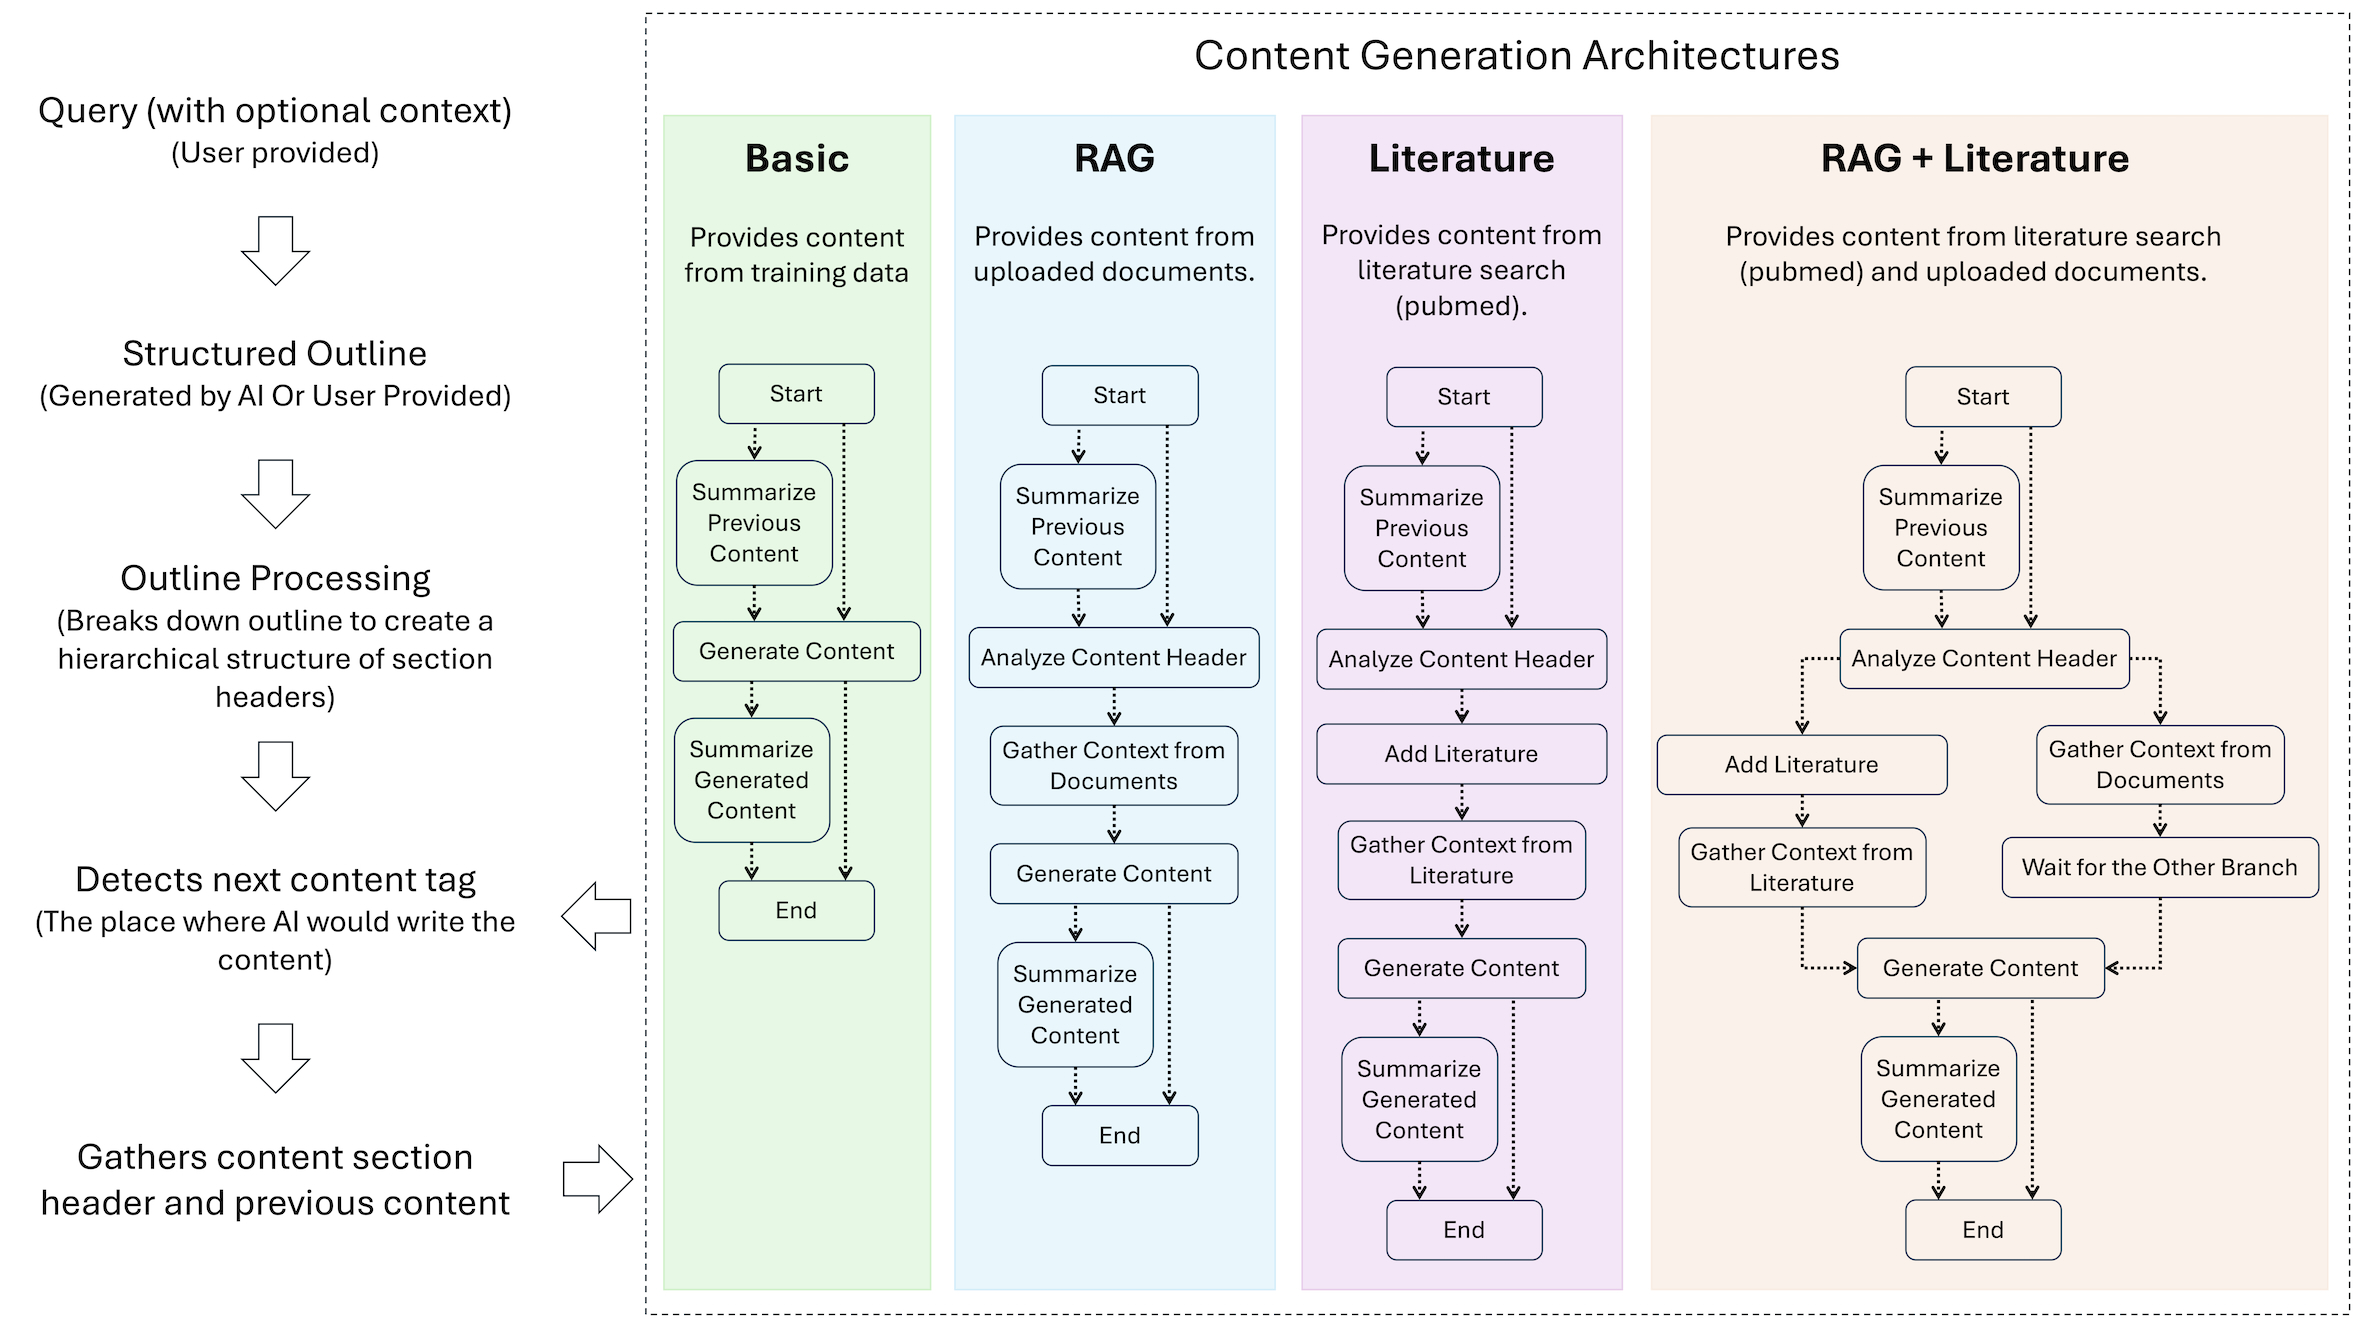
\includegraphics[width=1\linewidth]{workflows.jpg}
\caption{\label{fig:ai_workflow} Behind-the-scene user input processing steps and different AI workflows.}
\end{figure}

\begin{figure}
\centering
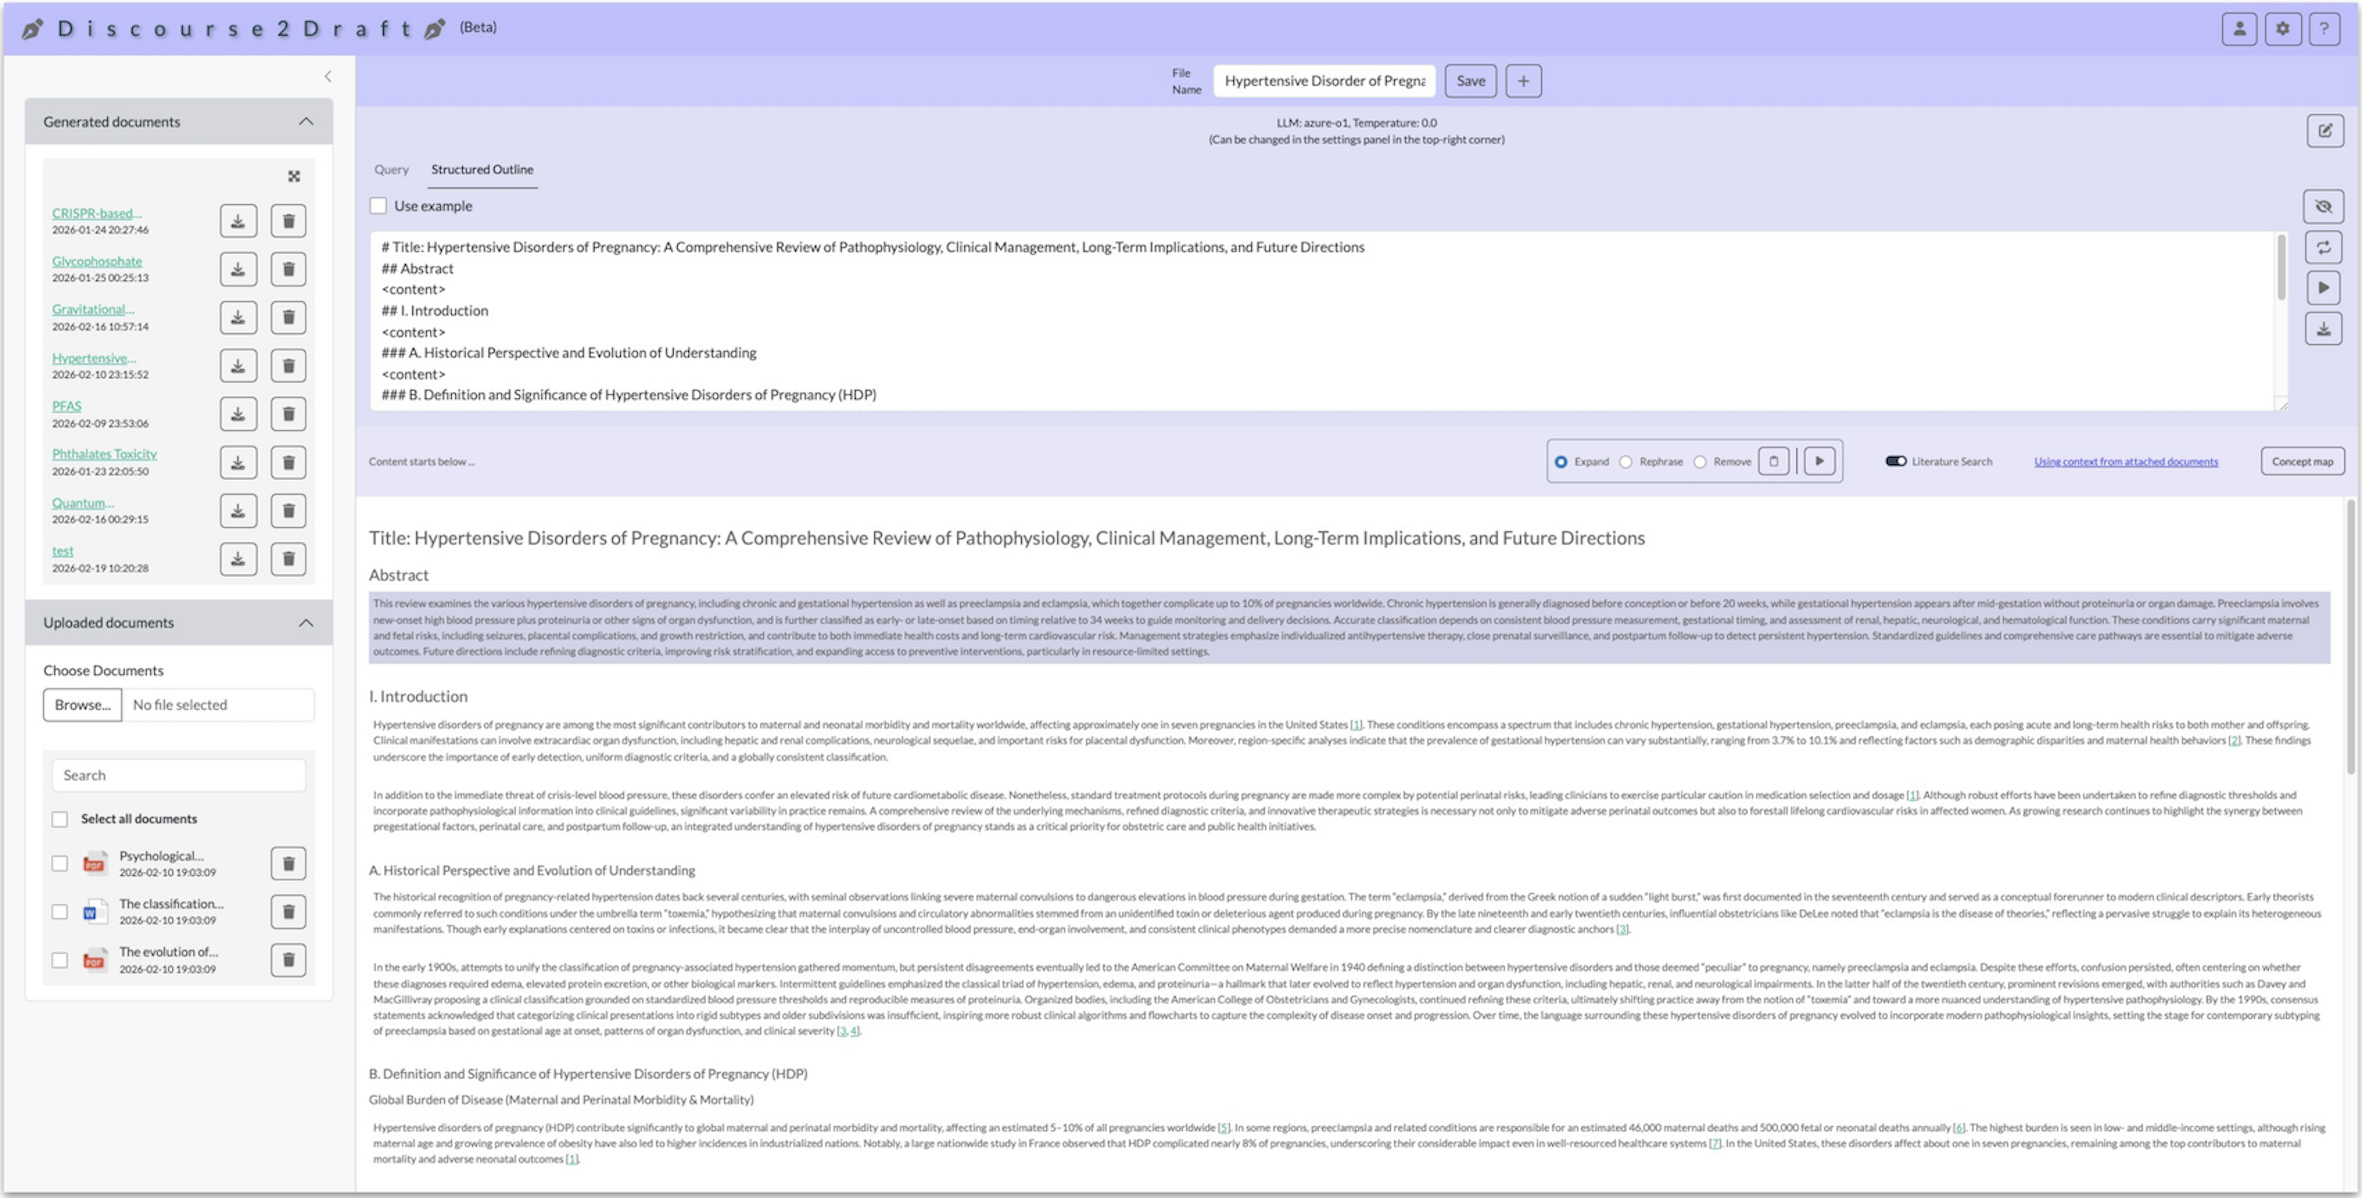
\includegraphics[width=1\linewidth]{app_screenshot.jpg}
\caption{\label{fig:app_screenshot}Content generation window of the app. The top left and bottom left panels show the generated and user uploaded files. The top right panel contains the outline. The bottom right panel contains the generated content.}
\end{figure}

\begin{figure}
\centering
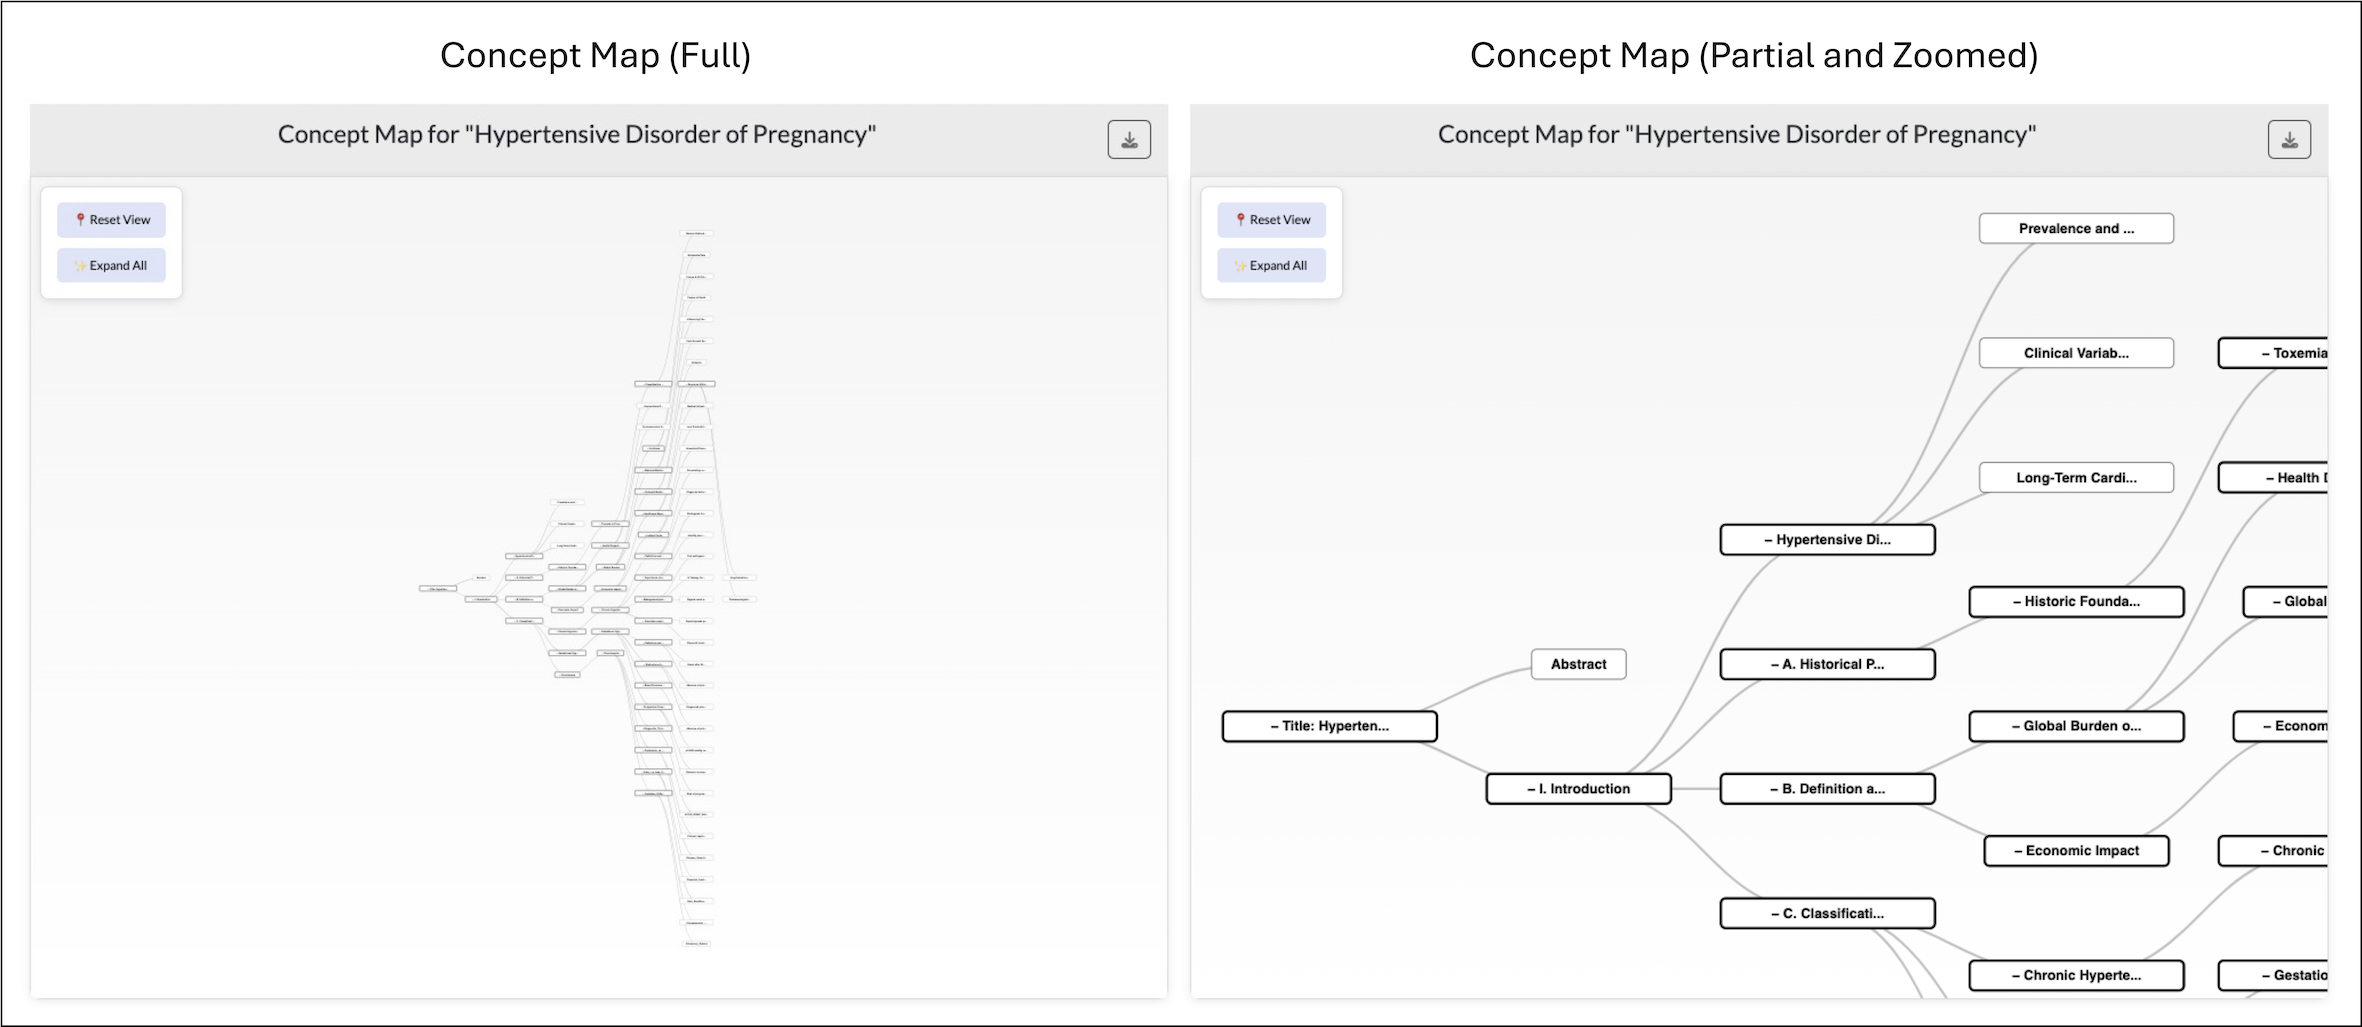
\includegraphics[width=1\linewidth]{concept_map.jpg}
\caption{\label{fig:concept_map}Concept map of a document generated by \appname{}.}
\end{figure}

\begin{figure}
\centering
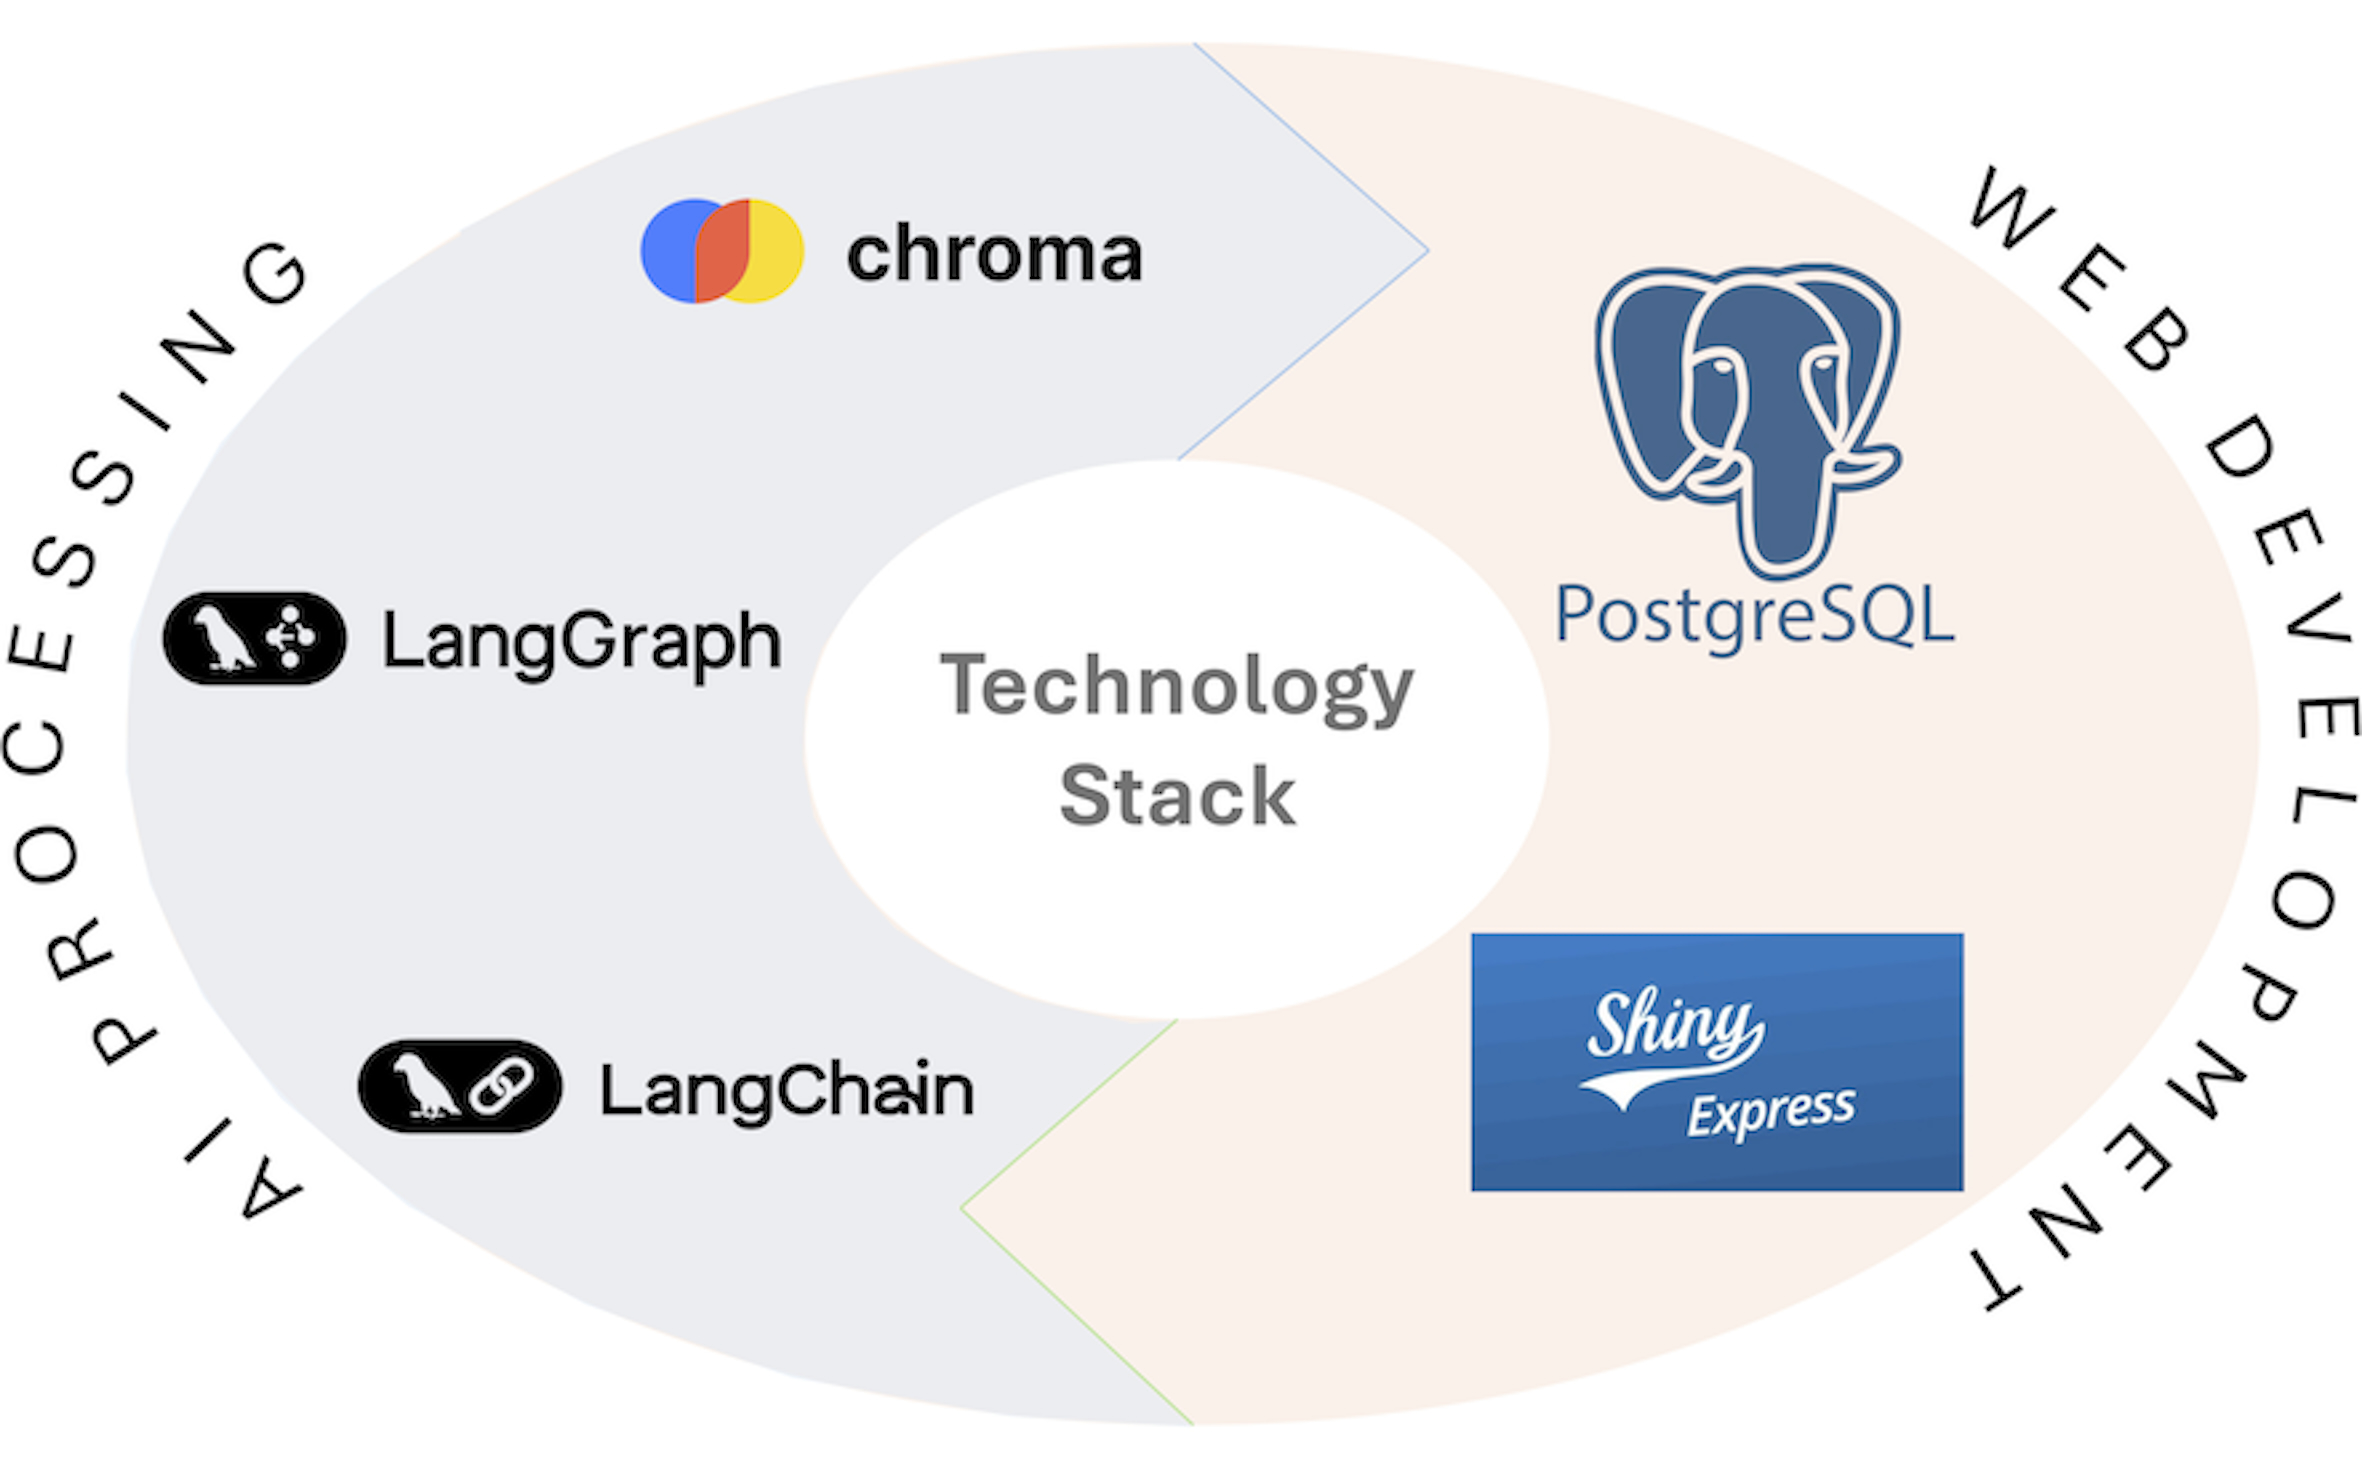
\includegraphics[width=0.7\linewidth]{tech_stack.jpg}
\caption{\label{fig:tech_stack} The technology stack used to develop the app.}
\end{figure}

\begin{figure}
\centering
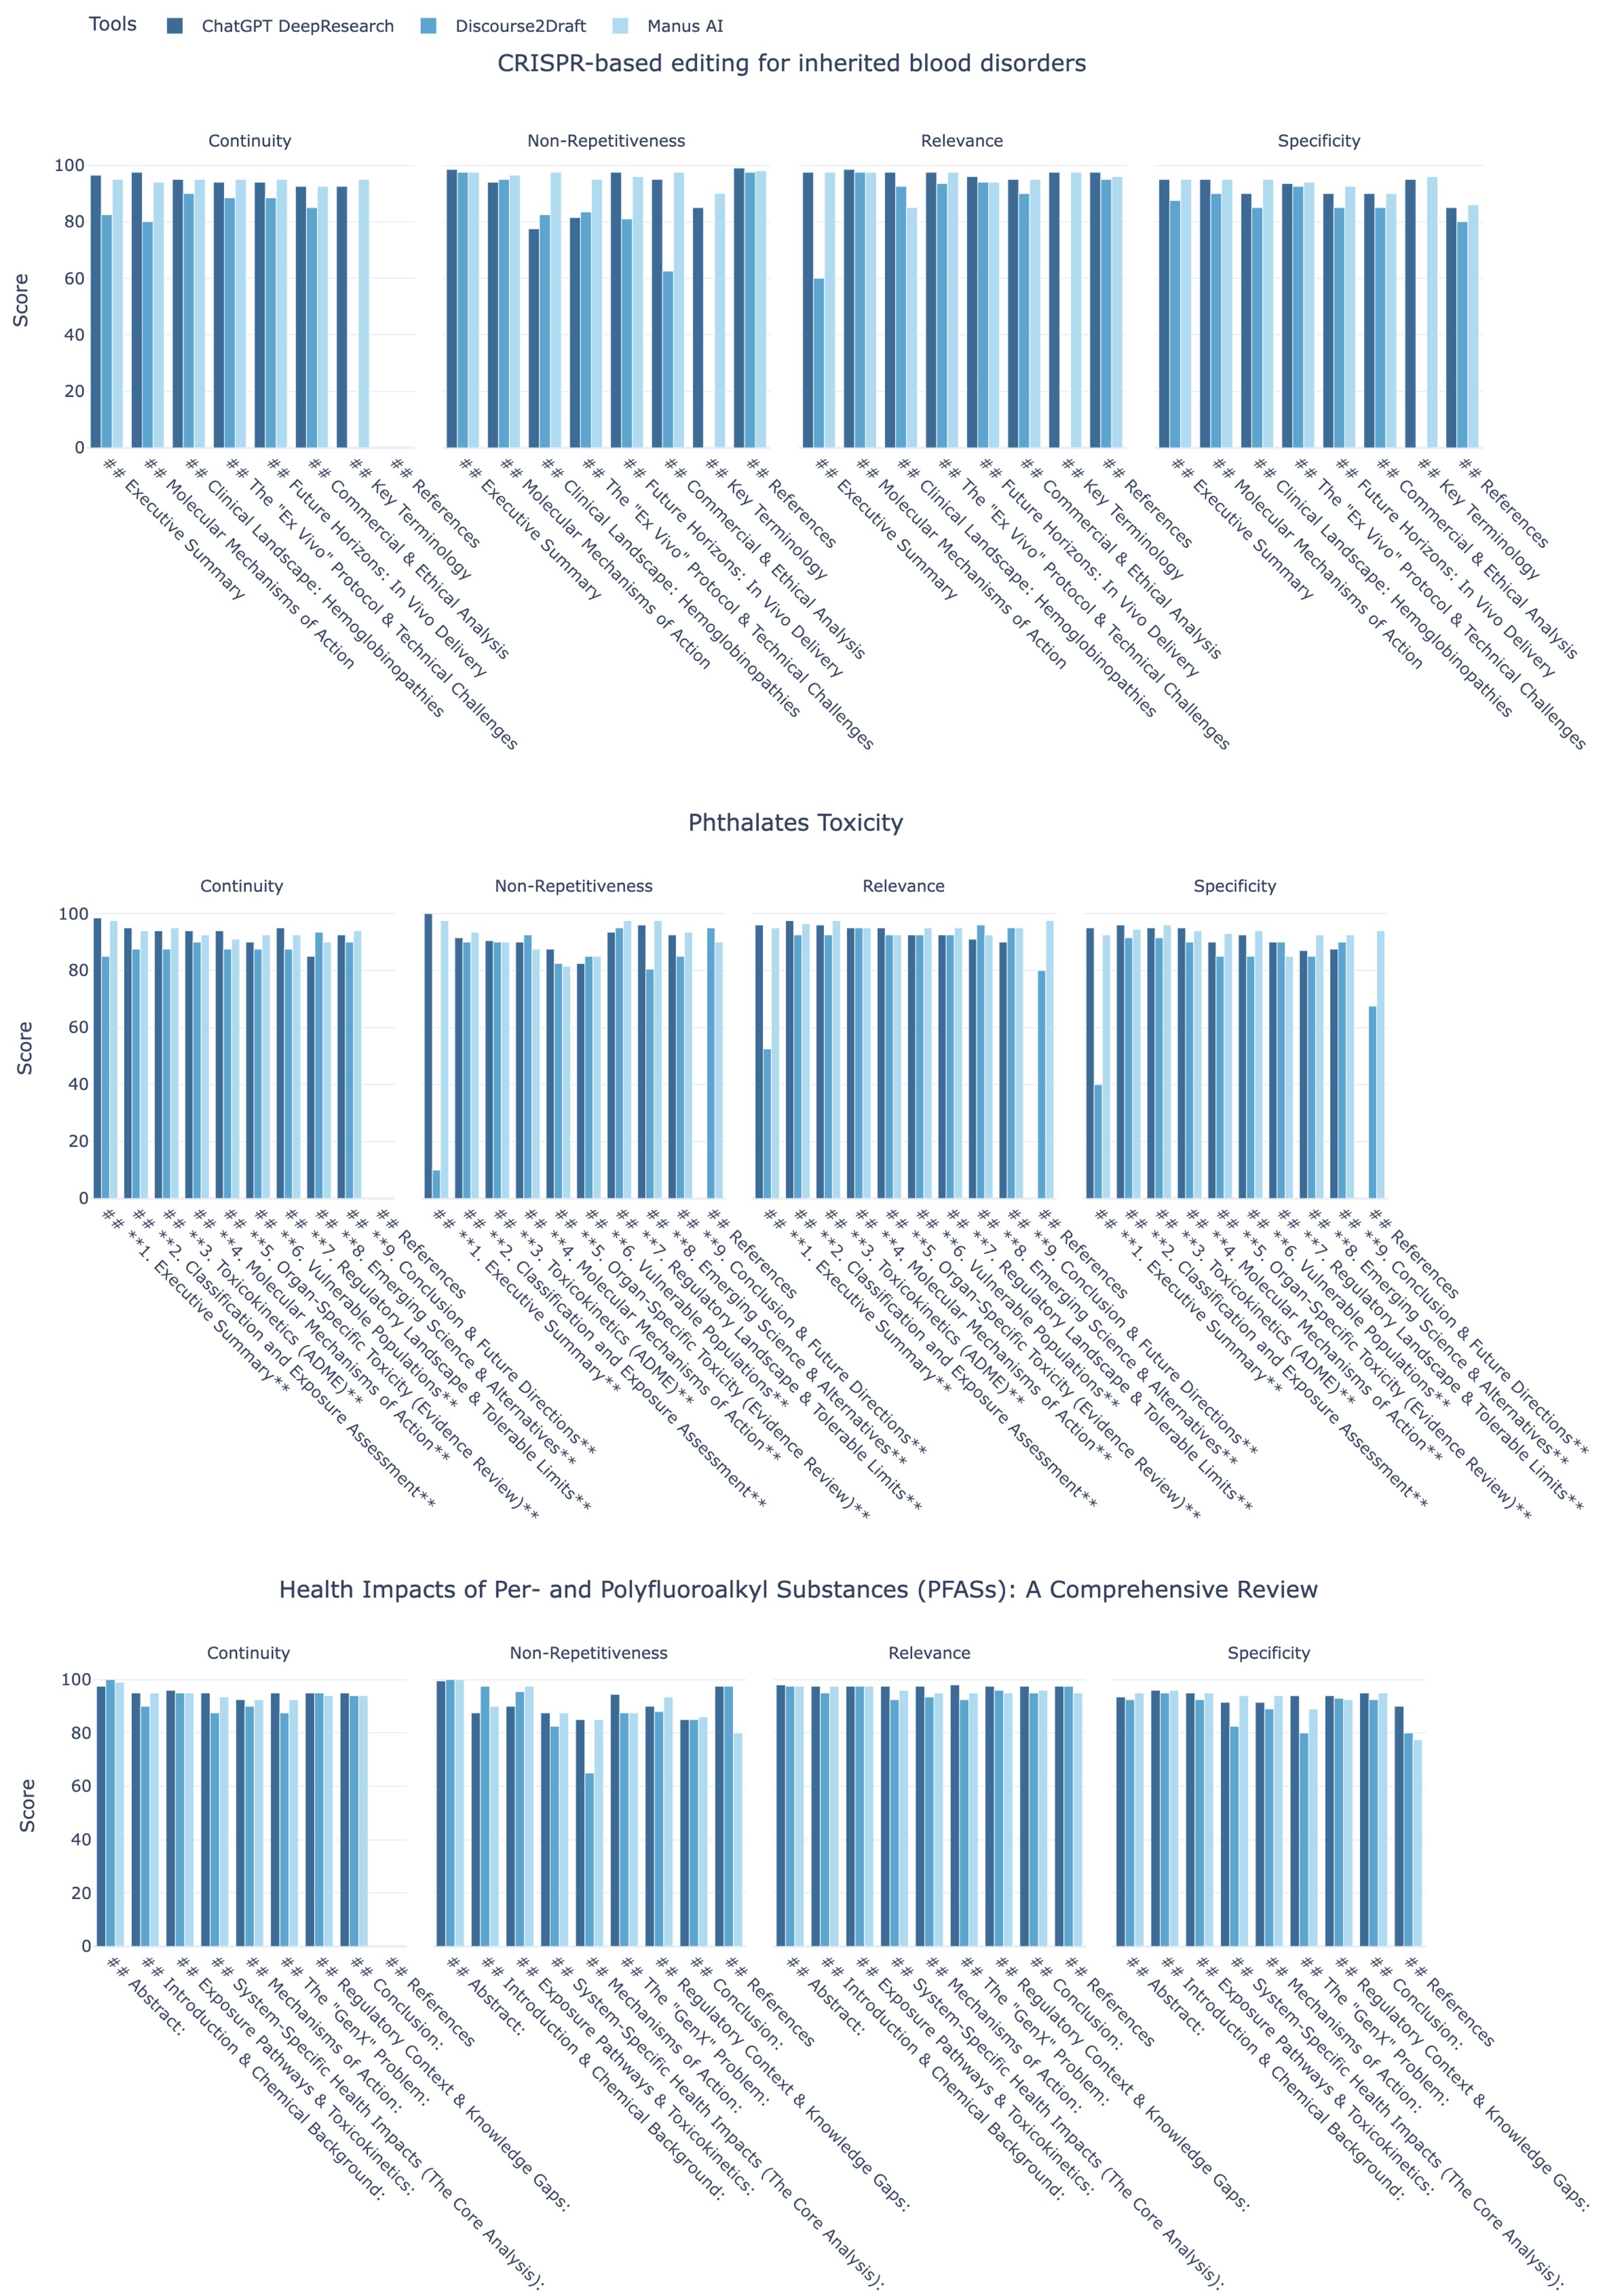
\includegraphics[width=1\linewidth]{eval_scores.jpg}
\caption{\label{fig:eval_scores}Evaluation scores.}
\end{figure}

\end{document}
